% Copyright (c) 2026 CorrectBrain
% SPDX-License-Identifier: MIT

\PassOptionsToPackage{dvipsnames,svgnames,x11names}{xcolor}
\documentclass[tikz,border=8pt]{standalone}
\usepackage{fontspec}
\usepackage{amsmath}
\usepackage{amssymb}
\usepackage{fontawesome5}
\usetikzlibrary{
    arrows.meta,
    positioning,
    calc,
    shapes,
    shadows,
    shadows.blur,
    decorations.pathmorphing,
    shapes.geometric,
    backgrounds,
    decorations.markings,
    decorations.pathreplacing,
    decorations.text,
    fit,
    shapes.misc,
    shapes.arrows,
    matrix,
    bending,
    3d,
    chains,
    intersections,
    shapes.symbols,
    svg.path,
    shapes.multipart,
    snakes,
    shapes.callouts,
    angles,
    quotes,
    fadings,
    patterns,
    patterns.meta
}

\renewcommand{\familydefault}{\sfdefault}

% --- STANDARD PALETTE ---
\providecolor{gold}{RGB}{212,175,55}
\providecolor{silver}{RGB}{192,192,192}
\providecolor{bronze}{RGB}{205,127,50}
\providecolor{darkblue}{RGB}{0,0,139}
\providecolor{lightblue}{RGB}{173,216,230}
\providecolor{darkgreen}{RGB}{0,100,0}
\providecolor{lightgreen}{RGB}{144,238,144}
\providecolor{darkred}{RGB}{139,0,0}
\providecolor{navy}{RGB}{0,0,128}
\providecolor{skyblue}{RGB}{135,206,235}
\providecolor{beige}{RGB}{245,245,220}
\providecolor{cream}{RGB}{255,253,208}

% --- CUSTOM COLORS ---
\definecolor{clienta}{RGB}{46, 204, 113}     % Green for Client A
\definecolor{clientb}{RGB}{155, 89, 182}     % Purple for Client B
\definecolor{darktext}{RGB}{47, 54, 64}      % Main text
\definecolor{warncolor}{RGB}{231, 76, 60}    % Red Warning
\definecolor{browserbg}{RGB}{220, 221, 225}  % Browser Chrome

\begin{document}
\begin{tikzpicture}[
    x=1cm, y=1cm,
    every node/.style={font=\sffamily},
    bubble/.style={draw=gray!30, fill=white, rounded corners=8pt, blur shadow={shadow opacity=15}, inner sep=10pt},
    browser/.style={fill=white, draw=gray!40, thick},
    chrome/.style={fill=browserbg}
]

% --- BACKGROUND (Pure White) ---
\fill[white] (-11.078,-9.752) rectangle (11.0843,11.7588);

% --- TITLE SECTION ---
\node[align=center, font=\Huge\bfseries\sffamily, text=darktext] at (0.0843,11.1588) {Fluid Layout Independence of Density Descriptors};
\node[align=center, font=\Large\sffamily, text=darktext!70] at (0.118,10.4792) {Why CSS \texttt{width: 50vw} changes nothing about the engine's \texttt{2x} source selection.};
\node[align=center, font=\Large\bfseries\sffamily, text=darktext] at (0.0843,9.1588) {Two Different Viewports, Same Hardware Density};

% ============================================================================
% --- DEVICE 1: DESKTOP MONITOR (USER A) ---
% ============================================================================
\node[font=\Large\bfseries\sffamily, text=clienta] at (-5,8.0361) {\faDesktop\ User A: 4K Retina Display};
\node[font=\bfseries\sffamily, text=darktext] at (-5,7.5361) {Hardware DPR = 2.0};

% Monitor Stand & Base Plate
\fill[left color=gray!50, right color=gray!20, rounded corners=3pt] (-6.5, -0.2) rectangle (-3.5, 0);
\fill[left color=gray!40, right color=gray!10] (-6, 0) -- (-4, 0) -- (-4.5, 1) -- (-5.5, 1) -- cycle;

% Monitor Bezel & Screen
\path[fill=black!85, rounded corners=6pt, drop shadow={opacity=0.3}] (-9.5, 1) rectangle (-0.5, 7.0);
\fill[white] (-9.2, 1.3) rectangle (-0.8, 6.7);

% Browser Window Chrome (Width = 7.0 units)
\fill[browserbg, rounded corners=3pt] (-8.5, 5.7) rectangle (-1.5, 6.3);
\fill[red!80!black] (-8.0, 6.0) circle (2pt);
\fill[yellow!80!black] (-7.7, 6.0) circle (2pt);
\fill[green!75!black] (-7.4, 6.0) circle (2pt);
\fill[white, rounded corners=2pt] (-7.0, 5.85) rectangle (-2.0, 6.15);
\node[font=\footnotesize, text=gray] at (-5, 6.0) {Window Width: 1800px};

% Browser Body
\fill[browser] (-8.5, 2.0) rectangle (-1.5, 5.7);

% Mathematically Correct 50vw Layout (Exactly 3.5 units wide, centered at x=-5)
\fill[clienta!10, draw=clienta, thick, dashed] (-6.75, 2.5) rectangle (-3.25, 4.5);
\node[font=\scriptsize\bfseries, text=clienta!80!black, align=center, text width=3.2cm] at (-5.0, 3.9) {CSS Layout:\\width 50vw};
\node[font=\scriptsize, text=darktext, align=center, text width=3.2cm] at (-5.0, 3.1) {Computed Width:\\\textbf{900px}};

% Downloads Label
\node[font=\small\bfseries, text=warncolor, fill=warncolor!10, draw=warncolor, rounded corners=4pt, inner sep=4pt] at (-5, -0.8) {Downloads: \texttt{image-2x.jpg}};


% ============================================================================
% --- DEVICE 2: HIGH-END MOBILE (USER B) ---
% ============================================================================
\node[font=\Large\bfseries\sffamily, text=clientb] at (5.0506,8.0866) {\faIcon{mobile-alt}\ User B: High-End Mobile};
\node[font=\bfseries\sffamily, text=darktext] at (5.0506,7.5866) {Hardware DPR = 2.0};

% Smartphone Bezel & Screen (Wider: 5.0 units total width)
\path[fill=black!85, rounded corners=12pt, drop shadow={opacity=0.3}] (2.5, -0.2) rectangle (7.5, 7.0);
\fill[white, rounded corners=8pt] (2.7, 0.0) rectangle (7.3, 6.8);
\fill[black, rounded corners=3pt] (4.2, 6.5) rectangle (5.8, 6.8);

% Browser Window Chrome (Width = 4.6 units)
\fill[browserbg, rounded corners=2pt] (2.7, 5.8) rectangle (7.3, 6.4);
\fill[white, rounded corners=2pt] (3.2, 5.95) rectangle (6.8, 6.25);
\node[font=\scriptsize, text=gray] at (5, 6.1) {Window Width: 400px};

% Browser Body
\fill[browser] (2.7, 1.5) rectangle (7.3, 5.8);

% Mathematically Correct 50vw Layout (Exactly 2.3 units wide, centered at x=5)
\fill[clientb!10, draw=clientb, thick, dashed] (3.85, 2.5) rectangle (6.15, 4.5);
\node[font=\scriptsize\bfseries, text=clientb!80!black, align=center, text width=2.1cm] at (5.0, 3.9) {CSS Layout:\\width 50vw};
\node[font=\scriptsize, text=darktext, align=center, text width=2.1cm] at (5.0, 3.1) {Computed Width:\\\textbf{200px}};

% Downloads Label
\node[font=\small\bfseries, text=warncolor, fill=warncolor!10, draw=warncolor, rounded corners=4pt, inner sep=4pt] at (5, -0.8) {Downloads: \texttt{image-2x.jpg}};


% ============================================================================
% --- EXPLANATION & TRANSITION ARROWS ---
% ============================================================================
\draw[-Latex, ultra thick, gray!70] (-5, -1.5) -- (-5, -2.5);
\draw[-Latex, ultra thick, gray!70] (5, -1.5) -- (5, -2.5);


% ============================================================================
% --- THE ARCHITECTURE PIPELINE (BOTTOM) ---
% ============================================================================
\node[align=center, font=\Large\bfseries, text=darktext] at (0, -3.2) {The Underlying Architecture Pipeline};

% Step 1: HTML Parsing (Center x=-6.8)
\path[fill=gray!10, draw=gray!40, thick, rounded corners=6pt, blur shadow] (-9.6, -7.5) rectangle (-4.0, -4.0);
\node[font=\large\bfseries, text=darktext] at (-6.8, -4.9) {1. HTML Parsing};
\node[font=\small, text=darktext, align=center, text width=5.0cm] at (-6.8, -6.1) {Engine encounters \texttt{<img>}\\sees \texttt{srcset="... 2x"}};

% Step 2: Network Dispatch (Center x=0)
\path[fill=orange!5, draw=orange, ultra thick, rounded corners=6pt, blur shadow] (-2.8, -7.5) rectangle (2.8, -4.0);
\node[font=\large\bfseries, text=orange!80!black] at (0, -4.9) {2. Network Dispatch};
\node[font=\small, text=darktext, align=center, text width=5.0cm] at (0, -6.1) {Engine queries OS DPR.\\DPR = 2.0. Engine \textbf{immediately}\\requests \texttt{image-2x.jpg}.};

% Step 3: CSS Computation (Center x=6.8)
\path[fill=red!5, draw=warncolor, thick, dashed, rounded corners=6pt, blur shadow] (4.0, -7.5) rectangle (9.6, -4.0);
\node[font=\large\bfseries, text=warncolor] at (6.8, -4.9) {3. CSS Computation};
\node[font=\small, text=darktext, align=center, text width=5.0cm] at (6.8, -6.1) {DOM calculates fluid layout.\\\texttt{width: 50vw} is applied.\\\textbf{(Too late to change image!)}};

% Flow Arrows Between Steps (with 3pt shorten gap)
\draw[-Latex, ultra thick, darktext, shorten <=3pt, shorten >=3pt] (-4.0, -5.75) -- (-2.8, -5.75);
\draw[-Latex, ultra thick, darktext, shorten <=3pt, shorten >=3pt] (2.8, -5.75) -- (4.0, -5.75);

% Timeline Brackets
\draw[thick, gray, decorate, decoration={brace, amplitude=15pt, mirror}] (-9.6, -7.8) -- (2.8, -7.8);
\node[font=\bfseries, text=darktext] at (-3.4, -8.5) {Pre-load Scanner Phase (Fast)};

\draw[thick, gray, decorate, decoration={brace, amplitude=15pt, mirror}] (4.0, -7.8) -- (9.6, -7.8);
\node[font=\bfseries, text=darktext] at (6.8, -8.5) {Rendering Phase (Slow)};

\end{tikzpicture}
\end{document}
